\subsection{Extended Log Likelihood Probability}

Log likelihood method of PID compares the measured DIRC signal to the expected signals for different particle hypotheses. The DIRC measures the arrival times $t_{i}$ and positions $(x_{i}, y_{i})$ of the $N$ Cherenkov photons detected on the photodetection plane. For each detected pixel the measured quantity can be a set of reconstructed Cherenkov angles (from the geometrical reconstruction) or hit time (see the time imaging reconstruction). The signals for all detected pixels are compared to the model, and the extended log likelihood probability $\log\mathcal{L}$ for a given charged particle hypothesis $h$ 
%($\log\mathcal{L}$) for different particle hypotheses 
($h = e, \mu, \pi, K, p$) can be 
defined as~\cite{staric2}:

\begin{equation}
\log\mathcal{L}_{h} = \sum_{i=1}^{N} \log \Big( \frac{S_{h}(x_{i}, y_{i}, t_{i}) + B_{h}(x_{i}, y_{i}, t_{i})}{N_{e}} \Big) + \log P_{N}(N_{e}),
\label{eq:ll}
\end{equation}

\noindent where $S_{h} (x_{i}, y_{i}, t_{i})$ is the signal distribution for the hypothesis $h$ and $B(x_{i}, y_{i}, t_{i})$ is the distribution of background, and $N_{e} = N_{h} + N_{B}$ is the expected number of detected photons, being a sum of the expected number of signal photons $N_{h}$ for hypothesis $h$ and the expected number of background photons, $N_{B}$. The second term in Eq.~\ref{eq:ll} is the Poisson probability to obtain $N$ photons if the mean is $N_{e}$.
%$P_{N}(N)$ is the probability to get the measured number of Cherenkov photons for this hypothesis based on the distribution of the number of expected photons.

For the geometrical reconstruction, the model is the expected value of the Cherenkov angle for the given particle type and momentum, smeared with the measured single photon Cherenkov angle resolution. The distribution is normalized to have the maximum value at 1 (Fig.~\ref{pic:spr} shows the simulated distributions of the Cherenkov angle normalized in the same way), so that the y axis shows the likelihood value. During the reconstruction, the log likelihood values for the reconstructed Cherenkov photons are summed up for all hit pixels (including all ambiguities). An example of the result is shown in Fig.~\ref{pic:sepLUT}.

\begin{figure}[!h]
\centering
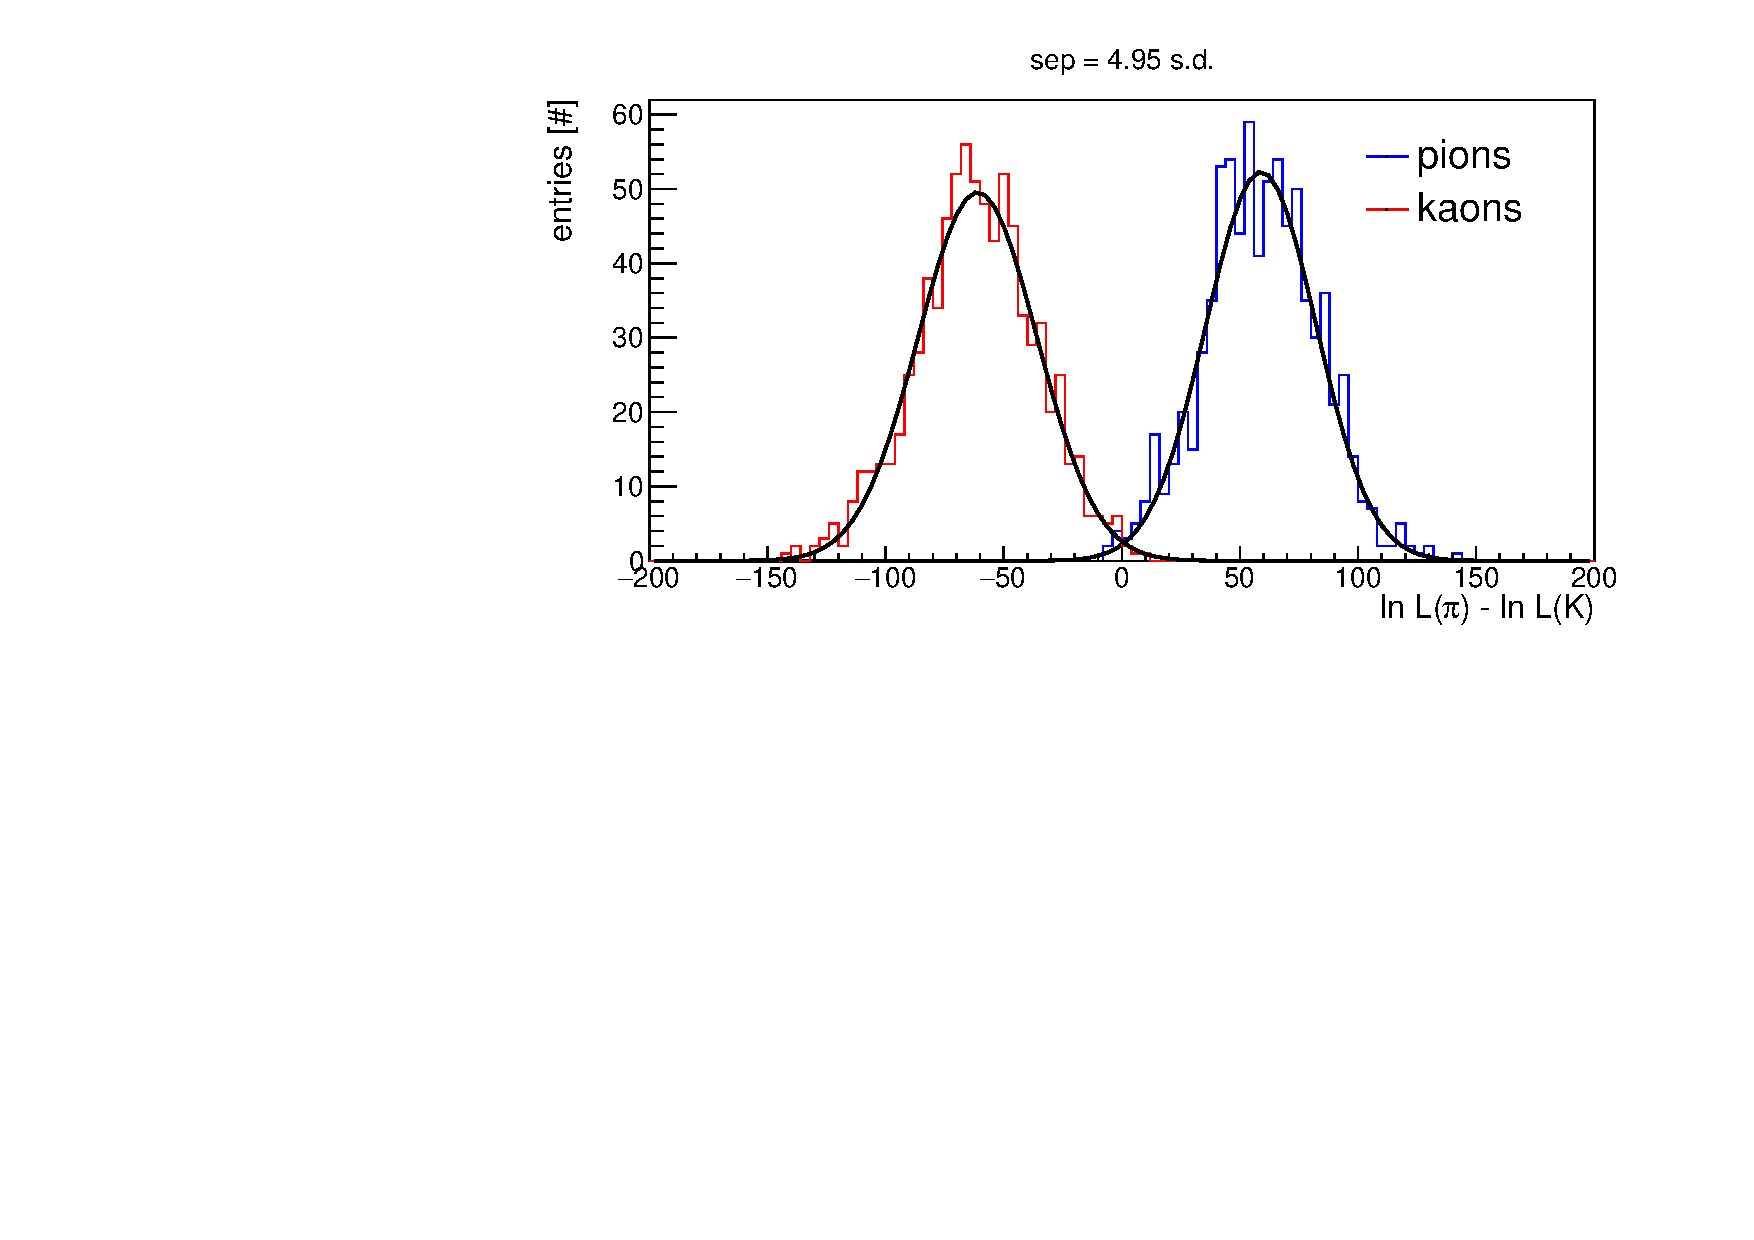
\includegraphics[clip, trim=0cm 0cm 0cm 0.7cm, width=0.8\textwidth]{pics/hLnDiff.pdf}
\caption{\label{pic:sepLUT}
Log likelihood difference between kaons (red) and pions (blue) with momenta of $4$ GeV/c, and direction defined by $\theta = 4^{\circ}$ and $\phi = 90^{\circ}$ is 4.95 s.d.
}
\end{figure}

The separation $S$ between two hypotheses can be calculated based on the difference in log likelihoods:

\begin{equation}
S = \frac{m_{1}-m_{2}}{1/2(\sigma_{1} + \sigma_{2})},
\end{equation}

\noindent where $m_{1}$ and $m_{2}$ are the mean values of the log likelihood difference for two hypotheses, and the denominator shows the average standard deviation assuming the log likelihood distributions are described by Gauss functions with $\sigma_{1}$ and $\sigma_{2}$.